\chapter{Background and Problem}

% - old ud-gf
% - newer naive approach - github + article 2017
%   - limitations
%   - performance


% Background to the assignment. Why is it relevant?
\section{Background}
\section{Problem}
% The formulation of the problem at hand and, the assignment. This should include an extended version of the scientific problem definition and references to knowledge within the area given in the thesis proposal.

% What has been done before and what remains to be done

% 2. Background & Problem
% - old ud-gf
% - newer naive approach - github + article 2017
%   - limitations
%   - performance

The current ud2gf implementation has some limitations. There are three main problems this work tries to fix.

The first problem is that it quickly becomes extremely slow for sentences with more than a couple of words and/or
when using large GF-grammars, e.g. GF-grammars containing Wordnet\cite{angelov2016predicting}. \\
The second problem is that if the structure differs too much between the representation of a sentence in UD format and as a GF tree, it is not possible to describe the required transformation in the current "labels file" language. See section \ref{sect:flex} below for more details. \\
The third problem is that it can sometimes be difficult to figure out why a rule in a labels-file is not firing, so it would be useful to have a debugging tool to help diagnosing such issues.


\subsection{Flexibility}\label{sect:flex}

As an example of a phrase that can be difficult to convert using the old gf2ud, let us consider the adjectival phrase "cute, fluffy and furry"
would be described in UD format as in Figures \ref{fig:ud_cute_text} and \ref{fig:ud_cute}.


\begin{figure}
    \begin{verbatim}
    1  cute  cute  ADJ  JJ  Degree=Pos  0  root  _  FUN=cute_A
    2  ,  ,  PUNCT  ,  _  3  punct  _  _
    3  fluffy  fluffy  ADJ  JJ  Degree=Pos  1  conj  _  FUN=fluffy_A
    4  and  and  CCONJ  CC  _  5  cc  _  FUN=and_Conj
    5  furry  furry  ADJ  JJ  Degree=Pos  1  conj  _  FUN=furry_A
    \end{verbatim}
    % \begin{tabular}{|c|c|c|c|c|c|c|c|c|c|}
    % \hline
    % 1 & cute & cute & ADJ & JJ & Degree\=Pos & 0 & root & \_ & FUN\=cute\_A \
    % \hline
    % 2 & , & , & PUNCT & , & \_ & 3 & punct & \_ & \_ \
    % \hline
    % 3 & fluffy & fluffy & ADJ & JJ & Degree\=Pos & 1 & conj & _ & FUN\=fluffy\_A \
    % \hline
    % 4 & and & and & CCONJ & CC & \_ & 5 & cc & \_ & FUN\=and\_Conj \
    % \hline
    % 5 & furry & furry & ADJ & JJ & Degree\=Pos & 1 & conj & \_ & FUN\=furry\_A \
    % \hline
    % \end{tabular}
    \caption{The phrase "cute, fluffy and furry" as a textual UD tree}
    \label{fig:ud_cute_text}
\end{figure}

\begin{figure}
    \centering
    % \begin{dependency}
  \begin{deptext}[column sep=0.4cm]
      cute \& , \& fluffy \& and \& furry \\
    {\tt ADJ}\&{\tt PUNCT}\&{\tt ADJ}\&{\tt CCONJ}\&{\tt ADJ} \\
  \end{deptext}
  \depedge{2}{1}{punct}
  \depedge{0}{2}{conj}
  \depedge{4}{3}{cc}
  \depedge{0}{4}{conj}
\end{dependency} \\
    % \includesvg{ud-annotatrix-corpus.svg}
    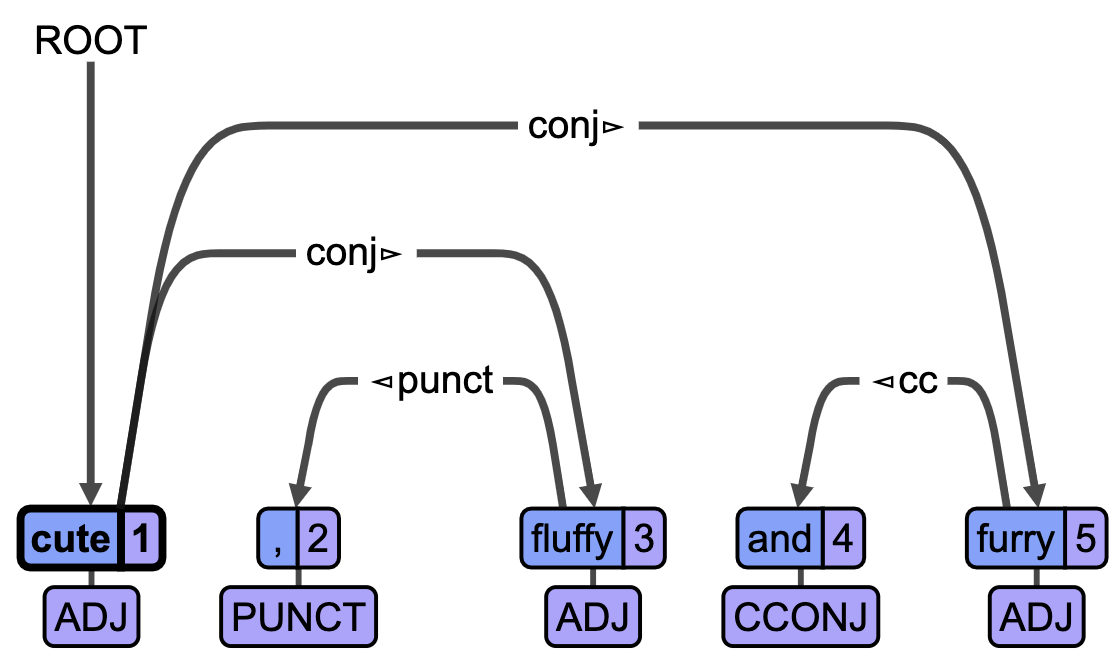
\includegraphics[width=0.7\textwidth]{figure/ud_cute.png}
    \caption{The phrase "cute, fluffy and furry" as a UD tree in graphical format}
    \label{fig:ud_cute}
\end{figure}
% \include{}

\begin{figure}
    \centering
    % \begin{dependency}
  \begin{deptext}[column sep=0.4cm]
      cute \& , \& fluffy \& and \& furry \\
    {\tt ADJ}\&{\tt PUNCT}\&{\tt ADJ}\&{\tt CCONJ}\&{\tt ADJ} \\
  \end{deptext}
  \depedge{2}{1}{punct}
  \depedge{0}{2}{conj}
  \depedge{4}{3}{cc}
  \depedge{0}{4}{conj}
\end{dependency} \\
    % \includesvg{ud-annotatrix-corpus.svg}
    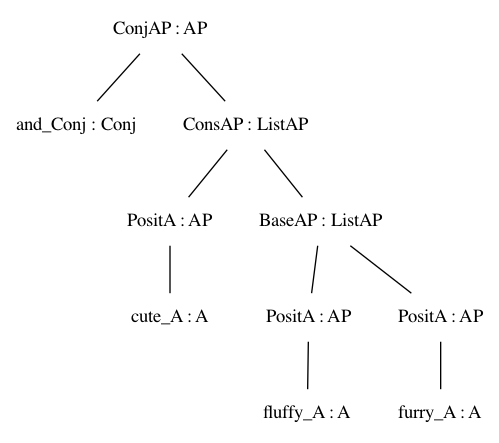
\includegraphics[width=0.7\textwidth]{figure/cute_gf.png}
    \caption{The phrase "cute, fluffy and furry" as a GF tree in graphical format. }
    \label{fig:gf_cute}
\end{figure}

The GF version of the same tree, shown in Figure \ref{fig:gf_cute}, would look like this:

\begin{verbatim}
ConjAP and_Conj (ConsAP (PositA cute_A)
                        (BaseAP (PositA fluffy_A) (PositA furry_A)))
\end{verbatim}
Here we can see that in UD, the word "cute" is in the root, while the conjunction "and" is at the bottom of the tree, while in GF the conjunction is a direct child of the root. This transformation can not be preformed by the simple single-layer transformations that are available in the current macro-system for labels files.

% Ideas:
%
% - Limits on how to transform trees - solution: extend language. currently hack using lambda calculus, but maybe better macros
%
% - Evaluate effectiveness of tool
%
% - (somewhere mention the performance boosts and analyse the complexity of it)

% This section is optional. It may be used if there is a need to describe the problem that you want to solve in more technical
% detail and if this problem description is too extensive to fit in the introduction.

% From elsewhere:
% - Background: GF \cite{ranta-2004}, UD \cite{nivre-etal-2016-universal},
%   - previous work: gf2ud \cite{kolachina-ranta-2016}, ud2gf \cite{kolachina-ranta-2017}
% - Describe the new algorithm
% - Extending the macro language
%   - Need for improvement: to match "fluffy and cute" needs 2 levels of nesting
%   - Solution: continuations
% - Case study: legal language

The translation described by a labels file is not one-to-one and there are often many possible GF trees that a UD tree could be translated to. The possible trees are currently ranked by completeness, as in how many of the words are included in the generated tree. However this ranking is incomplete and in case two possible trees, with the same GF category, cover the same words, an arbitrary tree will be chosen. A better choice could be to also check the linearization of these trees and rank those whose linearization is more similar to the original string higher. It would also be possible to completely exclude trees with differing linearization, but that would run counter to the goal of robustness.


% 3. The new algorithm
% - definitions
% - examples
% - how annotations work

% \section{Context}
% \todo[inline]{What's the difference between this and intro?}
% This work is mostly a continuation of the work in \cite{kolachina-ranta-2017}.

% A practical problem for which this tool can be useful can be found in \cite{listenmaa-etal-2021-towards}. In the Future Work section, under "Robust fall-back options", gf2ud is mentioned as a possible solution to making the parser more robust.

% % Use one or two relevant and high quality references for providing evidence from the literature that the proposed study indeed
% % includes scientific and engineering challenges, or is related to existing ones. Convince the reader that the problem addressed
% % in this thesis has not been solved prior to this project.

% Aim for the work. What should be accomplished?
\section{Goals and Challenges}

% try to preserve as much information as possible from the UD tree

% do this in an efficient way

% \todo[inline]{No longer relevant for final report?}

% \todo[inline]{Change this so it's clear that it has already been done}

1. Analyze algorithms and improve performance. The main challenge here is to find an algorithm for finding matching trees without exponential complexity on the number of children of a node in the UD tree.

2. Improve flexibility of macro language, allowing changing the structure of the trees while translating from GF to UD. One challenge here is in figuring out either how to change the algorithms to support these more advanced transformations or to find a way to allow them without needing to change the algorithms.

3. Write a debugging tool, which analyzes exactly what it is that prevents a rule in a labels-file from firing or what prevents that tree from being selected.
One challenge here is how to explain to the user the issue for all the possible things that can go wrong.
There is also an engineering challenge in making an algorithm that figures out what went wrong and why.
% either repeating the steps of the algorithm in order to find the issues or transforming the algorithm in a way that they can explain what went wrong

4. Document the version of the tool on which this work is based on, which had changed since what was written in \cite{kolachina-ranta-2017}


\subsection{Future work}

5. If there is time, update the algorithm to look at the linearization in order to try to select trees that match the original string as closely as possible and evaluate what difference this makes. This is only possible with improved performance from goal 1, but keeping it fast will still be a challenge. There are also some challenges here in how it should interact with the advanced macros in goal 2. We also need to handle when a GF tree has multiple linearizations, e.g. if it results in a conjugation table.

% % improve

% % Analyse the complexity of old and new algorithm, evaluate effectiveness of ...

% % Describe your contribution with respect to concepts, theory and technical goals. Ensure that the scientific and engineering
% % challenges stand out so that the reader can easily recognize that you are planning to solve an advanced problem.


% Limitations. What should be left out and why?
\section{Limitations}

Only the direction of converting UD trees to GF trees is studied here, because that is what was relevant to the application at hand. Furthermore, the two directions are almost completely independent in the implementation.

% I normalfallet behöver avgränsningarna inte motiveras.

% Limit the work mostly to what has already been done

% Har gjort:
%

%  \todo{why?}

% \todo[inline]{other limitations?}
